\documentclass[a4paper, 12pt]{article}

\usepackage{hyperref}
\usepackage{fullpage}
\usepackage[top=0.5in, bottom=1.5in, left=0.5in, right=0.5in, footskip=4em]{geometry}
\usepackage{amsmath}
\usepackage{fancyhdr}
\usepackage[usenames,dvipsnames]{xcolor}
\usepackage{pgfornament}

\usepackage[shortlabels]{enumitem}
\usepackage{xspace}
\usepackage{lastpage}
\usepackage{multicol}
\usepackage{blindtext}
\usepackage{titling}
\usepackage{standalone}
\usepackage{amsfonts}
\usepackage[framemethod=TikZ]{mdframed}
\usetikzlibrary{calc}
\usepackage{lineno}
\usepackage{amsthm}
\usepackage{amssymb}
\usepackage{mathtools}
\usepackage{datetime}
\usepackage[most]{tcolorbox}
\usepackage{cancel}
\usetikzlibrary{tikzmark, trees, backgrounds}
\usepackage{pgfplots}
\linenumbers
\usepackage{tikz-qtree}

%BEGIN_FOLD Commands
\newcommand{\half}{\frac{1}{2}}
\newcommand{\epv}[1]{\ensuremath{\left< #1 \right>}\xspace}
\newcommand{\variance}{\ensuremath{\text{Var}}}
\newcommand{\eout}{\ensuremath{E_\text{out}}\xspace}
\newcommand{\ein}{\ensuremath{E_\text{in}}\xspace}
\newcommand{\cx}{\ensuremath{\mathcal{X}}\xspace}
\newcommand{\cz}{\ensuremath{\mathcal{Z}}\xspace}
\newcommand{\real}{\mathbb{R}}
\DeclareSymbolFont{extraup}{U}{zavm}{m}{n}
\DeclareMathSymbol{\varheart}{\mathalpha}{extraup}{86}
\DeclareMathSymbol{\vardiamond}{\mathalpha}{extraup}{87}
\renewcommand{\heartsuit}{\textcolor{red}{\varheart}}
\renewcommand{\diamondsuit}{\textcolor{red}{\vardiamond}}
\newcommand{\definition}{\vspace{1em}\noindent\textbf{Def:} }
\newcommand{\theorem}{\vspace{1em}\noindent\textbf{Theorem:} }
\newcommand{\example}{\vspace{1em}\noindent\textbf{Example:} }
\newcommand{\solution}{\newline\noindent\textbf{Solution:} }
\newcommand{\predicate}{\vspace{0.25em}\noindent\textbf{Inductive Predicate:} }
\newcommand{\inductivestep}{\vspace{0.25em}\noindent\textbf{Inductive Step:} }
\renewcommand{\proof}{\vspace{0.5em}\noindent\textbf{Proof:} }
\newcommand{\lemma}{\vspace{1em}\noindent\textbf{Lemma:} }
\newcommand{\hint}{\textbf{Hint:} }
\newcommand{\basecase}{\vspace{0.25em}\noindent\textbf{Base Case:} }
\newcommand{\inductivehypothesis}{\vspace{0.25em}\noindent\textbf{Inductive Hypothesis:} }
\newcommand{\collorary}{\vspace{1em}\noindent\textbf{Collorary:} }
\newcommand{\qedd}{\qed\newline}
\newcommand{\kwd}[1]{\textcolor{blue}{\textbf{\underline{#1}}}}
\newcommand\ColorBox[2][]{%
	\stepcounter{mybox}%
	\node[draw=red!70!black,fill=red!20,align=left,#1] (box\themybox) {#2};
}
\newcommand{\expl}[2]{%
	\underset{\substack{\uparrow\\\mathrlap{\text{\hspace{-1em}#2}}}}{#1}}
\newcommand{\uexpl}[2]{%
	\overset{\substack{\mathrlap{\text{\hspace{-1em}#2}}\\\downarrow}}{#1}}
\newcommand{\st}{\text{ such that }}
\newcommand{\R}{\textcolor{red}{R}}
\newcommand{\sumn}{\sum^n_{i=0}}
\newcommand{\sumxn}{\sum^n_{x=0}}
\newcommand{\red}[1]{\textcolor{red}{#1}}
\newcommand{\blue}[1]{\textcolor{blue}{#1}}
%\newcommand{\qed}{\ensuremath{\blacksquare}}
%END_FOLD
\newcommand{\sidenote}[1]{\textcolor{gray}{#1}}

%BEGIN_FOLD miscellaneious default
\makeatletter
% Make a copy of macros responsible for entering display math mode
\let\start@align@nopar\start@align
\let\start@gather@nopar\start@gather
\let\start@multline@nopar\start@multline
% Add the "empty line" command to the macros
\long\def\start@align{\par\start@align@nopar}
\long\def\start@gather{\par\start@gather@nopar}
\long\def\start@multline{\par\start@multline@nopar}
\makeatother
\setlength{\columnsep}{1cm}
%opening
\setlength{\abovedisplayskip}{-\baselineskip}%
\setlength{\abovedisplayshortskip}{\abovedisplayskip}%

\pagestyle{fancy}
\renewcommand{\headrulewidth}{0pt}
\lfoot{\small{\course}: Week \weekno}
\rfoot{\small{\thetitle}}
\rhead{}
\cfoot{\pgfornament[height=1em, ydelta=-0.4em]{17} \thepage of \pageref{LastPage}  \pgfornament[height=1em, ydelta=-0.4em]{18}}

\DeclareMathOperator{\sign}{sign}
\newcommand{\vect}[1]{\ensuremath{\mathbf{#1}}\xspace}

\tikzstyle{every picture}+=[remember picture]
\newcommand{\bwgrid}[1]{
	\def \aaa #1
	
	\foreach \y in {0,1,2} {
		\foreach \x in {0,1,2} {
			\pgfmathsetmacro{\clr}{\aaa[\x][\y]}
			%\message{aaa \clr}
			\definecolor{MyColor}{rgb}{\clr,\clr,\clr}
			\path[fill=MyColor] (\x,\y) rectangle ++(1,1); 
		}
	}
	\draw[step=1cm,very thin] (0,0) grid (3,3);	
}

\setenumerate{label=\alph*.)}
\definecolor{db}{RGB}{100,65,23}

%END_FOLD

\newcommand{\course}{Discrete Math}
\title{Counting}
\newcommand{\weekno}{7}

\begin{document}
\begin{center}
	\textcolor{orange}{\textsc{\course}}\\
	\huge\textbf{\textsc{\thetitle}}\\
	\small\textcolor{gray}{Last updated:\, \today \, \currenttime}\\
	\pgfornament[width=0.7\textwidth, color=white!30!black]{88}
\end{center}


\begin{multicols}{2}
	\section*{Two Rules of Counting}
		Count (1) \kwd{everything} (2) \kwd{exactly once}. There is really no fixed rule to do it. It's all essentially common sense. It is not hard but this is really something that can not be taught. You will need to practice it a little bit to be good at it. 

	
	\section*{Boring Definition}
	\definition \kwd{Set} is an \emph{unordered} collection of item. The order doesn't matter. Duplicates are not allowed.
	
	For example, the set $\{3,2,1\}$ and the set $\{1,2,3\}$ are the same set.
	
	\definition \kwd{Cardinality} of a set is the number of items in the set. We use $|S|$ to denote the cardinality of set $S$.
	
	For example, the cardinality of the set $S = \{1,2,3\}$ is $|S| = 3$.
	
	\definition \kwd{Sequence} is an \emph{ordered} collection of item. The order matters.
	
	For example, the sequence
	\[
		(1,2,3) \ne (3,2,1).
	\]
	Furthermore, dupicate elements are allowed ex: $(1,1,2)$ is also a sequence.
	
	\definition A \kwd{permutation} of a set $S$ is a sequence that contains every element in $S$ exactly once.
	 
	For example, let $S = \{a,b,c\}$
	\[
		(a,b,c) \text{ is a permutation of } S
	\]
	\[
		(b, a, c) \text{ is also a permutation of } S
	\].

	

	\section*{Product Rule}
	Consider counting how many ways you can have a meal in a day. You have the following choices for breafast
	\[
		B = \{\text{Jok, Kao mun kai, Boiled Rice, Pancake}\}
	\]
	Then the following choice for Lunch
	\[
		L = \{\text{Noodles, Som tum, Omlette Rice}\}
	\]
	Then the following choices for dinner
	\[
		D = \{\text{Boat Noodles, Chicken Basil} \}
	\]
	
%	You can make a tree out of this
%	
%	\begin{tikzpicture}[grow'=right, every node/.style={draw, circle}]
%		\node {}
%			child{
%				node{B1} 
%					child{
%						node {L1}
%					}
%					child{
%						node{L2}
%					}
%					child{
%						node{L3}
%					}
%			}
%			child{
%				node{B2}
%				child[dashed]{}
%				child[dashed]{}
%				child[dashed]{}
%			}
%			child{
%				node{B3}
%			}
%			child{
%				node{B4}
%			};
%	\end{tikzpicture}
	
	Then the number of way you can have these meal in a day is
	\[
		\text{\# Meal} = |B|\times |L| \times |D|
	\]
	
	This is the common sense number one called the product rule.
	
	Here is some excercise you can do:
	
	\example How many password of 8 character no numbers are?
	\solution $26^8$
	
	\example How many license plate of the type NNCCNNN are?
	\solution $10\times10 \times 44 \times 44 \times 10^4$
	
	\example Counting IPv4 Addresses.
	\solution $256^4$
	
	\example Counting Bacteria. Bacteria-algae DNA contains about $10^5$ links. Each link has 4 possibilities.
	\solution $4^{10^5}$ a lot.
	
	\example How many ways are there to place knight bishop and pawn on an $8\times 8$ chessboard such that no two share the same row nor column.
	\solution $8 \times 8 \times 7 \times 7 \times 6 \times 6$
	
	\example How many ways are there to arrange $10$ different numbers?
	\solution Since there are 10 different ways to pick the first number, then 9 different ways to pick the second number and so on. The number of ways to arrange 10 numbers is
	\[
		10\times 9 \times 8 \times \ldots \time 3 \times 2 \times 1 = 10!
	\]
	
	\example How many binary string of 32 bits are there?
	\solution $2^{32}$
	
	\section*{Counting Another}
	\example How many ways are there to pick numbers from a list of $32$ distinct number.
	\solution Let us not count this directly. Instead, we can form a one to one map between the binary string of 32 bits number and the numbers we picked. All we need to do is to have the i-th digit represent whether we pick such number(1) or not(0).  Since we can count the number of binary string of 32 bits and the numbers we picked, the cardinality of both sets are equal. Thus, there are $2^{32}$ ways to pick numbers from $32$ distinct number.
	
	This is a very powerful technique which needs some imagination. You will see some more difficult example later.
	

	\section*{Sum Rule}
	Common sense: If you count multiple things, count each one add them up.
	
	\example How many alphanumeric password are there that is 6-8 character long?
	\solution All we need to do is count how many 6 character password are there then 7 then 8. After that we just need to add them up. So the answer is $62^6 + 62^7 + 62^8$.
	
	\section*{Subtraction Rule}
	Another common sense: If you overcount, subtract off.
	
	\example Let us count the number of 8 alphanumeric password with at least 1 number.
	\solution If we count all the password then we will overcount the one with no number in. But, that can be counted easily. So, the number of password with at least 1 character is $62^8 - 52^8$.
	
	\example How many binary string are there that start with 1 \emph{or} end with 00.
	\solution We could count the nubmer of binary strings that start with 1. That is just $2^9$. Then we can count the number of binary strings that end with 00: $2^8$. But, if we just add the two we would double count those then we would double count those that start with 1 \emph{and} end with 00. So all we need is just count those that start with 1 \emph{and} end with 00 ($2^7$) then subtract it off from the first sum. So the answer is
	\[
	2^9 + 2^8 - 2^7
	\]

	\section*{Division Rule}
	Common sense: If you count everything twice(or anything with multiple factor) all you need to do is divide.
	
	\example We can count the number of people in the room by counting the nubmer of ears then divide by 2.
	
	\example How many ways are there to place 2 rooks on the chessboard such that they do not share the same row nor column?
	\solution If the two rooks are different then it is easy. It would be just $8\cdot8\cdot7\cdot7$. However, this counts each of what we want twice. So all we need to do is divide the answer by two. So the answer is
	\[
	\frac{8\cdot8\cdot7\cdot7}{2}
	\]
	
	\example How many ways are there to place 2 rooks and 2 bishop on the chessboard such that none of them share the same row nor column?
		\solution If all the chess pieces are different that is easy to count $(8\cdot7\cdot6\cdot5)^2$. We then need to divide by 2 for double counting the rook. Then divide it by another two for double counting the bishop. This yields the final answer of
		\[
		\frac{(8\cdot7\cdot6\cdot5)^2}{2\cdot 2}
		\]
	
	\example Let us consider sitting 10 people in a round table. How many ways are there for them to sit. If all adjacent ppl are the same then we consider them to be the same way.
	\solution We can translate this in to the problem of counting the permutation of 10 people. Then we assign the first person to seat no 1 the second to seat no 2 ans so on. There are $10!$ permutaions. However, such mapping count each way of sitting by 10 times. For example, $(10,9,8,\ldots,1)$ and $(1,10,9,8,\ldots,2)$ results in the same seating but they both got counted in $10!$. So, we need to divide the $10!$ by 10. So the answer is
	\[
		10!/10 = 9!
	\]
	
	\example Now what if there are two people out of the 10 demand that they must sit next to each other. How many way of sitting are there?
	\solution For this we need to be a bit creative. We can just lump the two picky people(A, B) together. Then we have 9 object to arrange in a circle $9!/9$. Then, we can unpack the two people. There are two ways to do that: A sits before B or B sits before A. So, the answer is
	\[
		9!/9 \times 2
	\]
	
	\section*{Choosing}
	One of the most common theme that occur in counting problem is \emph{choosing}. But, essentially this is just a division rule in disguise.
	
	\example How many ways are there to \emph{choose} 5 yoyo from 22 flavor?
	\solution So first we can arrange the 22 yoyo (22!). But we overcount the permutation of the 5 yoyo we pick by a factor of $5!$. We also overcount the permutation of the $22-5$ flavors we don't pick by $(22-5)!$. So, the number of way to choose $5$ flavors from $22$ flavors is just
	\[
		\frac{22!}{5!(22-5)!} \equiv {22 \choose 5} 
	\]
	
	The problem of choosing comes up so often that we invent a new notation for them
	\[
		\frac{n!}{k! (n-k)!} \equiv {n \choose k}
	\]
	which reads $n$ choose $k$ which is the number of choosing $k$ things from $n$ things ignoring the order. Normally, when we face the problem that involve choosing items we just use $n$ choose $k$, we normally don't do the division rule. But, it is good that you know it is just a division rule in disguise.
	
	\example How many ways are there to give 3 yoyo of the same flavor to 8 students?
	\solution All we need is to choose 3 students from 8 students to give the yoyo choose 3 student from the 8 student $\displaystyle {8 \choose 3}$.
	
	\example Now what if the 3 yoyo are all of different flavor?
	\solution Well we can first choose the 3 student from 8 students to give yoyo $\displaystyle {8 \choose 3}$. Then for the 3 student we can arrange them so we can assign yoyo. That's another $3!$. So the answer is\[
		{8 \choose 3} \times 3!
	\]
	
	\example Now how about if I have 2 cola yoyo and 1 grape yoyo?
	\solution We can choose 2 studnet to give the 2 cola $\displaystyle {8 \choose 2}$. Then we choose 1 student from the 7 student. So\[
		{8 \choose 2} \times 7
	\]
	
	
	\example How many squares are there if we have 5 vertical line and 7 horizontal lines.
	\solution Each different square is form by 2 vertical lines and 2  horizontal lines so the nubmer of square is then\[
		{5 \choose 2}{7 \choose 2}
	\]
	
	\example How many 8 character(uppercase) password are there such that no to character are used twice?
	\solution $\displaystyle {26 \choose 8}$
	
	\section*{Inclusion-Exclusion 3 Ways}
	
	If we want to find the size of $|A \cup B \cup C|$,
	\begin{itemize}
		\item The first attempt would be to just add up $|A|+|B|+|C|$ but this means we over count the intersection like mad.
\begin{center}
				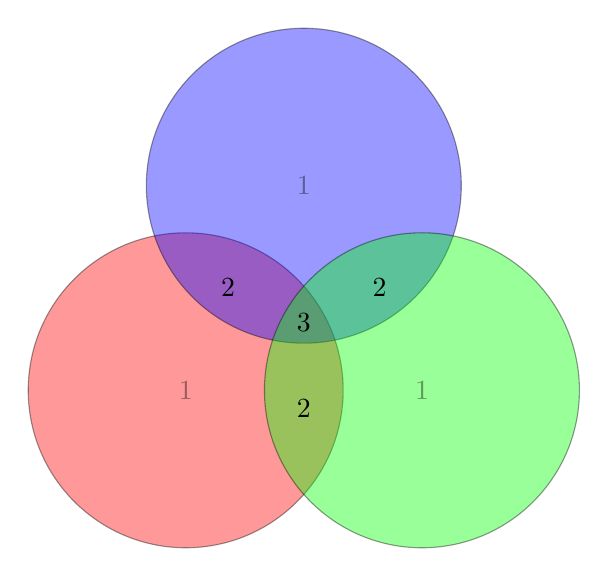
\begin{tikzpicture}
			\tikzset{venn circle/.style={draw,circle,minimum width=4cm,fill=#1,opacity=0.4}}
			
			\node [venn circle = red] (A) at (0,0) {1};
			\node [venn circle = blue] (B) at (60:3cm) {1};
			\node [venn circle = green] (C) at (0:3cm) {1};
			\node[left] at (barycentric cs:A=1/2,B=1/2 ) {2}; 
			\node[below] at (barycentric cs:A=1/2,C=1/2 ) {2};   
			\node[right] at (barycentric cs:B=1/2,C=1/2 ) {2};   
			\node[] at (barycentric cs:A=1/3,B=1/3,C=1/3 ){3};
			\end{tikzpicture} 
\end{center}
		\item The second attempt we would be subtracting off the intersection that is
		\[
		 |A|+|B|+|C| - |A \cap B| - |A \cap C| - | B \cap C|
		 \]
		 But, this creates another trouble since we subtract off the center(the insection of the three) three times which means we are left with
\begin{center}
			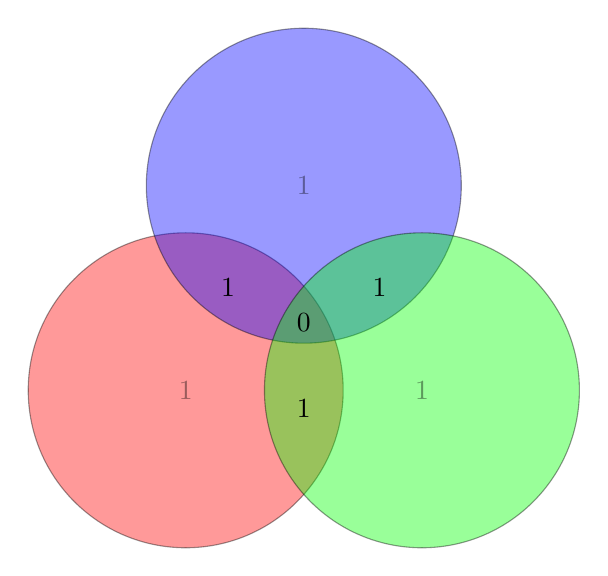
\begin{tikzpicture}
		\tikzset{venn circle/.style={draw,circle,minimum width=4cm,fill=#1,opacity=0.4}}
		
		\node [venn circle = red] (A) at (0,0) {1};
		\node [venn circle = blue] (B) at (60:3cm) {1};
		\node [venn circle = green] (C) at (0:3cm) {1};
		\node[left] at (barycentric cs:A=1/2,B=1/2 ) {1}; 
		\node[below] at (barycentric cs:A=1/2,C=1/2 ) {1};   
		\node[right] at (barycentric cs:B=1/2,C=1/2 ) {1};   
		\node[] at (barycentric cs:A=1/3,B=1/3,C=1/3 ){0};
		\end{tikzpicture}
\end{center}
		\item But this is very easy to fix since all we need to do is to \emph{add} the intersection of the three back. Specifically, 
		\begin{align*}
				|A \cup B \cup C|  =& |A|+|B|+|C|\\ 
				&- |A \cap B| - |A \cap C| - | B \cap C|\\
				& + |A \cap B \cap C|
		\end{align*}
		which gives us exactly what we want
					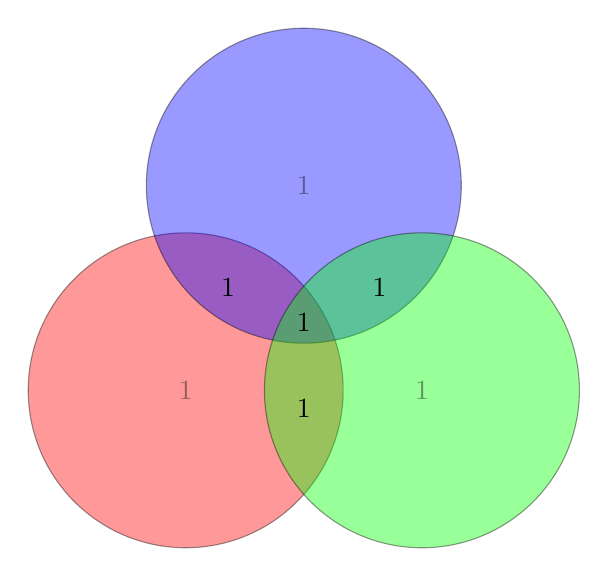
\begin{tikzpicture}
					\tikzset{venn circle/.style={draw,circle,minimum width=4cm,fill=#1,opacity=0.4}}
					
					\node [venn circle = red] (A) at (0,0) {1};
					\node [venn circle = blue] (B) at (60:3cm) {1};
					\node [venn circle = green] (C) at (0:3cm) {1};
					\node[left] at (barycentric cs:A=1/2,B=1/2 ) {1}; 
					\node[below] at (barycentric cs:A=1/2,C=1/2 ) {1};   
					\node[right] at (barycentric cs:B=1/2,C=1/2 ) {1};   
					\node[] at (barycentric cs:A=1/3,B=1/3,C=1/3 ){1};
					\end{tikzpicture}
 
	\end{itemize}
	\example How many permutation of the set $\{0,1,2,\ldots, 9\}$ has 42 or 04, or 60.
	\solution $9! + 9! + 9! - 8! -8! -8! + 7!$
	
	\section*{Sticks and Stones}
	\example Consider the problem of splitting $20$ identical yoyo to $10$ student. Such that everyone gets at least one yoyo.
	\solution$\displaystyle {19 \choose 9}$
	
	\example How about now, some kids do not behave so well so those bad kids don't get the yoyo. How many ways are there to split 20 identical yoyo to 10 students?
	\solution $\displaystyle {29 \choose 9}$
	
	
	\example There are 20 books on the shelf. How many ways are there to select 6 books so that no two adjacent book are selected?
	\solution $\displaystyle {20-6+1 \choose 6}$ 
	
	\section*{Random Problem}
	\example How many 12 bit string are there that doesn't have 01?
	\solution 13.
	
	\example How many binary questions you can ask to distinguish 5 items?
	\solution $2^{5-1} -1$.
	
	\example Suppose the pizza shop have 9 toppings, how many ways are there to order 3 pizza?
	\solution GLHF.
	
	\example The three deck of cards in 1409 are mixed up. Assuming that the same card from the different deck is distinguishable how many ways are there to arrage these cards?
	\solution GLHF
	
	\example Let us consider a square grid. You start at (0,0) then the treasure is at (30,40). On each step you can either go up 1 or go right 1. How many ways are there to get the reasure?
	\solution GLHF
	%\example How many ways are there to get the treasure and walk
	
	\section*{Binomial Theorem}
	Let us consider the following polynomial
	\[
		(a+b)^5
	\]
	
	We want to know the coefficient in front of the term $a^2b^3$. We can consider the multiplication
	\[
		(a+b)_1(a+b)_2(a+b)_3(a+b)_4(a+b)_5 
	\]
	
	To get $a^2b^3$ all you need to do is count how many way are there to pick two brakets to pick and $a$ from so the coefficient is $\displaystyle {5 \choose 2}$
	
	The same principle can be applied for a general case of\[
		(a+b)^n
	\]
	and you want to find the coefficent in front of $a^k b^{n-k}$. This is just $\displaystyle {n \choose k}$. With this we can write
	\[
		(a+b)^n = \sum_{k=0}^{n} {n \choose k} a^k b^{n-k}
	\]
	
	This is called binomial theorem. But, do not bother memorizing it though you can get it from the first principle in 1 minute.
	
	As an exercise try to figure out the coefficient in front of $a^2 b^3 c^5$ in
	\[
		(a + b + c)^{10}
	\]

	\section*{Combinatoric Proof}
	
	As you may find in many of the example above that you find a different way to get the answer. Counting the same thing using different methods has to give us the same number if we count it correctly. This is actually one of my favorite kind of proof.
	
	For example, let us count the number of ways to pick $k$ from $n$ people in the room. Assuming that one of the person in the room is Alice.
	
	One way to count this is as simple as the number of ways to choose $k$ people from $n$ people\[
	{n \choose k}.
	\]
	
	Another way to count this is to say that we can either pick or not pick Alice. If we pick alice then we just need to choose $k-1$ people from $n-1$ people. But if we don't pick alice then we need to choose $k$ people from $n-1$ people. If we add the two then we have the number of ways to choose $k$ people from $n$ people. This means the number of ways to choose  is
	\[
		{n-1\choose k-1} + {n-1 \choose k}
	\]
	
	The two ways are counting the same thing so they must be equal. So, by just this reasoning we have obtain Pascal's identity.
	\[
		{n \choose k} = {n-1\choose k-1} + {n-1 \choose k}
	\]
	The reason it is called the pascal identity since this is exactly how you get each number on the Pascal's triangle. (Wikipedia it if you don't know what it looks like)
	
	
	Let us look at a more colorful one
	
	\theorem\[
		\sum_{r=0}^{n} {n \choose r} {2n \choose n-r} = {3n \choose n}
	\]
	
	\proof If you try to do this with algebra you will probably give up after three terms. Induction doesn't help much either. Let us do a combinatoric proof them.
	
	Let us try to count the number of ways to pick $n$ yoyo from a jar of $3n$ distinguishable yoyo(let us say you mark them all with numbers) which comprises of $n$ cola yoyo, $n$ grape yoyo, $n$ pineapple yoyo.
	
	First way to compute it is that we do not even care what the colors are so the number of ways is
	\[
		{3n \choose n}
	\] 
	
	Now, if we are about the color then we know that we can choose $r = 0,1,\ldots,n$ cola yoyo first. There are $\displaystyle {n \choose r}$ ways to choose $r$ cola yoyo. Then all we need to do is to get $n-r$ yoyo from $2n$ non-cola yoyo. So, the number of ways is
	\[
		\sum_{r=0}^{n} {n \choose r} {2n \choose n-r}
	\]
	
	Since we are counting the same thing the two quantity must be equal
	\[
	\sum_{r=0}^{n} {n \choose r} {2n \choose n-r} = {3n \choose n}
	\]
	\qed

	\section*{Relations}
	
	\definition A function $f:A \to B$ is called \emph{injective} if for all element in $B$ there is \emph{at most} one element in $A$ maps to it.
	
	\definition A function $f:A \to B$ is called \emph{surjective} if for all element in $B$ there is \emph{at least} one element in $A$ maps to it.
	
	\definition A function $f:A \to B$ is called \emph{bijective}/\emph{one-to-one} if for all element in $B$ there is \emph{exactly} one element in $A$ maps to it. In other words, the function is bijective if and only if the function is both surjective and injective.
	
	\example Let us consider a function $f$ which maps $A = \{a,b,c\}$ to  $B=\{1,2,3\}$.
	\begin{center}
		
		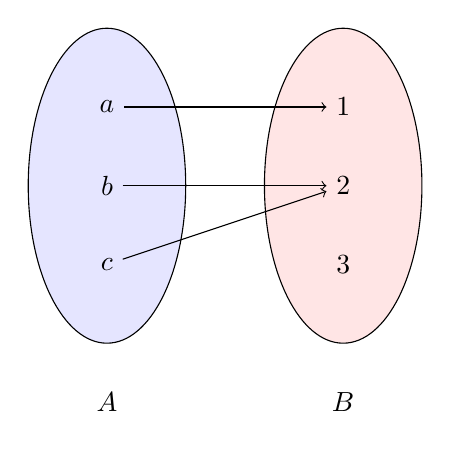
\begin{tikzpicture}
		\node(a) {$a$};
		\node(b) [below of = a] {$b$};
		\node(c) [below of = b] {$c$};
		\begin{scope}[on background layer]
		\draw[fill=blue!10!white] (b) ellipse (1cm and 2cm) node [below,yshift=-2.5cm] {$A$};
		\end{scope}
		
		
		\node(n1) [right of = a, xshift=2cm]{1};
		\node(n2) [below of = n1] {2};
		\node(n3) [below of = n2] {3};
		\begin{scope}[on background layer]
		\draw[fill=red!10!white] (n2) ellipse (1cm and 2cm) node [below,yshift=-2.5cm] {$B$};
		\end{scope}
		
		\draw[->] (a) -- (n1);
		\draw[->] (b) -- (n2);
		\draw[->] (c) -- (n2);
		
		\end{tikzpicture}
	\end{center}
	
	This function is not injective since $2$ has both $b$ and $c$ maps to it.
	
	Also, this function is not surjective since $3$ has nothing maps to it.
	
	\example Let us consider a function $g$ which maps $A = \{a,b,c\}$ to  $B=\{1,2,3,4\}$.
	\begin{center}
		
		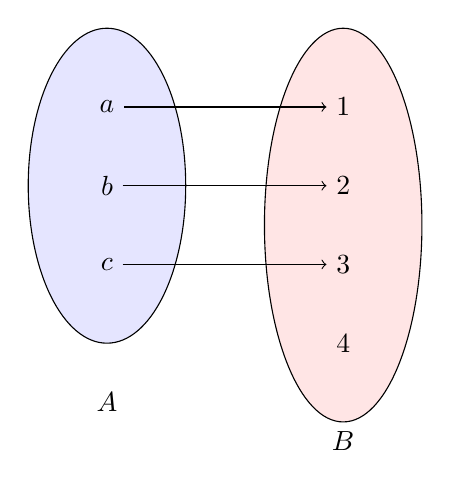
\begin{tikzpicture}
		\node(a) {$a$};
		\node(b) [below of = a] {$b$};
		\node(c) [below of = b] {$c$};
		\begin{scope}[on background layer]
		\draw[fill=blue!10!white] ($(a)!0.5!(c)$) ellipse (1cm and 2cm) node [below,yshift=-2.5cm] {$A$};
		\end{scope}
		
		
		\node(n1) [right of = a, xshift=2cm]{1};
		\node(n2) [below of = n1] {2};
		\node(n3) [below of = n2] {3};
		\node(n4) [below of = n3] {4};
		\begin{scope}[on background layer]
		\draw[fill=red!10!white] ($(n2)!0.5!(n3)$) ellipse (1cm and 2.5cm) node [below,yshift=-2.5cm] {$B$};
		\end{scope}
		
		\draw[->] (a) -- (n1);
		\draw[->] (b) -- (n2);
		\draw[->] (c) -- (n3);
		
		\end{tikzpicture}
	\end{center}
	
		The function $g$ is injective since every element in $B$ has at either 1 or zero element in A maps to it.
		
		The function $g$ is not surjective since there is nothing maps to $4$.
		
		
	\example Let us consider a function $h$ which maps $A = \{a,b,c,d\}$ to  $B=\{1,2,3\}$.
	\begin{center}
		
		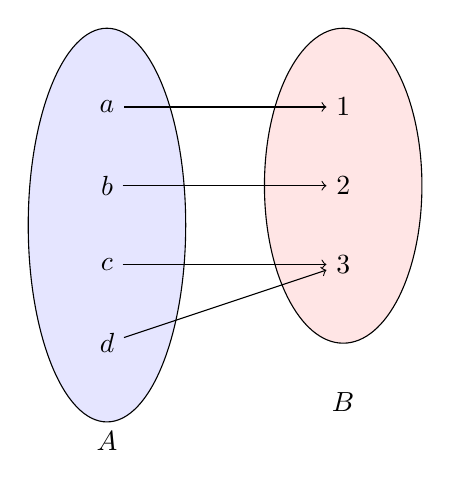
\begin{tikzpicture}
		\node(a) {$a$};
		\node(b) [below of = a] {$b$};
		\node(c) [below of = b] {$c$};
		\node(d) [below of = c] {$d$};
		\begin{scope}[on background layer]
		\draw[fill=blue!10!white] ($(b)!0.5!(c)$) ellipse (1cm and 2.5cm) node [below,yshift=-2.5cm] {$A$};
		\end{scope}
		
		
		\node(n1) [right of = a, xshift=2cm]{1};
		\node(n2) [below of = n1] {2};
		\node(n3) [below of = n2] {3};
		\begin{scope}[on background layer]
		\draw[fill=red!10!white] ($(n1)!0.5!(n3)$) ellipse (1cm and 2cm) node [below,yshift=-2.5cm] {$B$};
		\end{scope}
		
		\draw[->] (a) -- (n1);
		\draw[->] (b) -- (n2);
		\draw[->] (c) -- (n3);
		\draw[->] (d) -- (n3);
		\end{tikzpicture}
							
	\end{center}
	
	The function $h$ is not injective since both $c$ and $d$ map to 3.
		
	The function $h$ is surjective since there is every element in $B$ has something maps to it.
					

	\example Let us consider a function $q$ which maps $A = \{a,b,c\}$ to  $B=\{1,2,3\}$.
	\begin{center}
		
		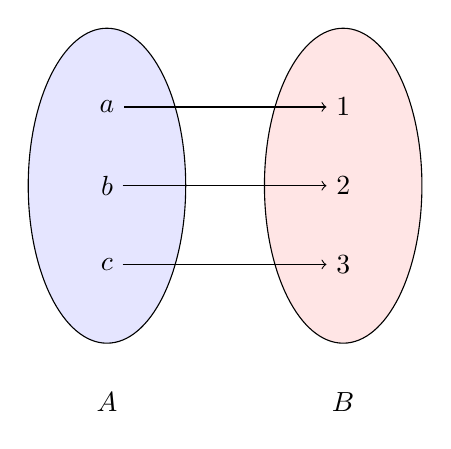
\begin{tikzpicture}
		\node(a) {$a$};
		\node(b) [below of = a] {$b$};
		\node(c) [below of = b] {$c$};
		\begin{scope}[on background layer]
		\draw[fill=blue!10!white] ($(a)!0.5!(c)$) ellipse (1cm and 2cm) node [below,yshift=-2.5cm] {$A$};
		\end{scope}
		
		
		\node(n1) [right of = a, xshift=2cm]{1};
		\node(n2) [below of = n1] {2};
		\node(n3) [below of = n2] {3};
		\begin{scope}[on background layer]
		\draw[fill=red!10!white] ($(n1)!0.5!(n3)$) ellipse (1cm and 2cm) node [below,yshift=-2.5cm] {$B$};
		\end{scope}
		
		\draw[->] (a) -- (n1);
		\draw[->] (b) -- (n2);
		\draw[->] (c) -- (n3);
		\end{tikzpicture}
		
	\end{center}
	
	The function $q$ is injective all element in $B$ has at most one element in $A$ maps to it.
	
	The function $q$ is surjective since there is every element in $B$ has something maps to it.
	
	Therefore, $q$ is bijective.
	
	
	
\end{multicols}


\end{document}
